\documentclass{article}
\usepackage{ctex}
\usepackage{fancyhdr}
\usepackage{extramarks}
\usepackage{amsmath}
\usepackage{amsthm}
\usepackage{amsfonts}
\usepackage{tikz}
\usepackage[plain]{algorithm}
\usepackage{algpseudocode}
\usepackage{extarrows}
\usepackage{indentfirst}

\usepackage[titletoc]{appendix}
\usepackage{pythonhighlight}
\usepackage{listings}
\usepackage[framed,numbered,autolinebreaks,useliterate]{mcode}

\usetikzlibrary{automata,positioning}

%
% Basic Document Settings
%

\topmargin=-0.45in
\evensidemargin=0in
\oddsidemargin=0in
\textwidth=6.5in
\textheight=9.0in
\headsep=0.25in

\linespread{1.1}

\pagestyle{fancy}
\lhead{\hmwkAuthorName}
\chead{\hmwkClass\ : \hmwkTitle}
\rhead{}
\lfoot{\lastxmark}
\cfoot{\thepage}

\renewcommand\headrulewidth{0.4pt}
\renewcommand\footrulewidth{0.4pt}

\setlength\parindent{2em}

%
% Create Problem Sections
%



\setcounter{secnumdepth}{0}
\newcounter{partCounter}
\newcounter{homeworkProblemCounter}
\setcounter{homeworkProblemCounter}{1}
\nobreak\extramarks{Problem \arabic{homeworkProblemCounter}}{}\nobreak{}

%
% Homework Problem Environment
%
% This environment takes an optional argument. When given, it will adjust the
% problem counter. This is useful for when the problems given for your
% assignment aren't sequential. See the last 3 problems of this template for an
% example.
%


%
% Homework Details
%   - Title
%   - Due date
%   - Class
%   - Section/Time
%   - Instructor
%   - Author
%

\newcommand{\hmwkTitle}{插值与多项式近似}
\newcommand{\hmwkDueDate}{May, 2022}
\newcommand{\hmwkClass}{数值分析作业}
\newcommand{\hmwkClassTime}{}
\newcommand{\hmwkClassInstructor}{}
\newcommand{\hmwkAuthorName}{\textbf{葛雨辰  201800150053}}

%
% Title Page
%

\title{
    \vspace{2in}
    \textmd{\textbf{\hmwkClass:\ \hmwkTitle}}\\
    \normalsize\vspace{0.1in}\small{Due\ on\ \hmwkDueDate\ }\\
    \vspace{0.1in}\large{\textit{\hmwkClassInstructor\ \hmwkClassTime}}
    \vspace{3in}
}

\author{\hmwkAuthorName}
\date{}

\renewcommand{\part}[1]{\textbf{\large Part \Alph{partCounter}}\stepcounter{partCounter}\\}

%
% Various Helper Commands
%

% Useful for algorithms
\newcommand{\alg}[1]{\textsc{\bfseries \footnotesize #1}}

% For derivatives
\newcommand{\deriv}[1]{\frac{\mathrm{d}}{\mathrm{d}x} (#1)}

% For partial derivatives
\newcommand{\pderiv}[2]{\frac{\partial}{\partial #1} (#2)}

% Integral dx
\newcommand{\dx}{\mathrm{d}x}

% Alias for the Solution section header
\newcommand{\solution}{\textbf{\large Solution}}

% Probability commands: Expectation, Variance, Covariance, Bias
\newcommand{\C}{\mathrm{C}}
\newcommand{\D}{\mathrm{D}}
\newcommand{\E}{\mathrm{E}}
\newcommand{\U}{\mathrm{U}}
\newcommand{\Z}{\mathbb{Z}}
\newcommand{\R}{\mathbb{R}}
\newcommand{\Q}{\mathbb{Q}}
\newcommand{\N}{\mathbb{N}}
\begin{document}

\maketitle

\pagebreak
\section{1. 序言}

本章节研究插值与多项式逼近问题,\textbf{不考虑导数时有}Lagrange插值多项式法,Nevile迭代插值法与Newton插值法。\textbf{考虑导数时有}Hermite插值多项式法。

首先声明以下所有程序都\textbf{按照方法名称命明},变量含义自明。

\section{2. 用Lagrange,Nevile与Newton插值计算3.1节3c题}

\subsection{2.1 运行程序与结果分析}
    
    发现3.1节3c题与3.3节1d题目数据相似,则擅自在3.1节3c题加入3.3节1d题目的导数值,由此也可以加入Hermite插值进行比较。(自然,Lagrange,Nevile与Newton插值照常比较,无需使用导数值。)

    分别用Lagrange,Nevile与Newton插值去逼近$f(0.25)$处的值,运行程序的结果如下。其中第一个与第三个得到插值多项式与在$f(0.25)$处的逼近值;第二个得到的是迭代矩阵,在右下角即为逼近值。第四个得到迭代矩阵(同样在右下角即为逼近值)以及插值多项式与在$f(0.25)$处的逼近值。四个程序都计算了CPU运行时间。
    \begin{figure}[h]
    \centering
    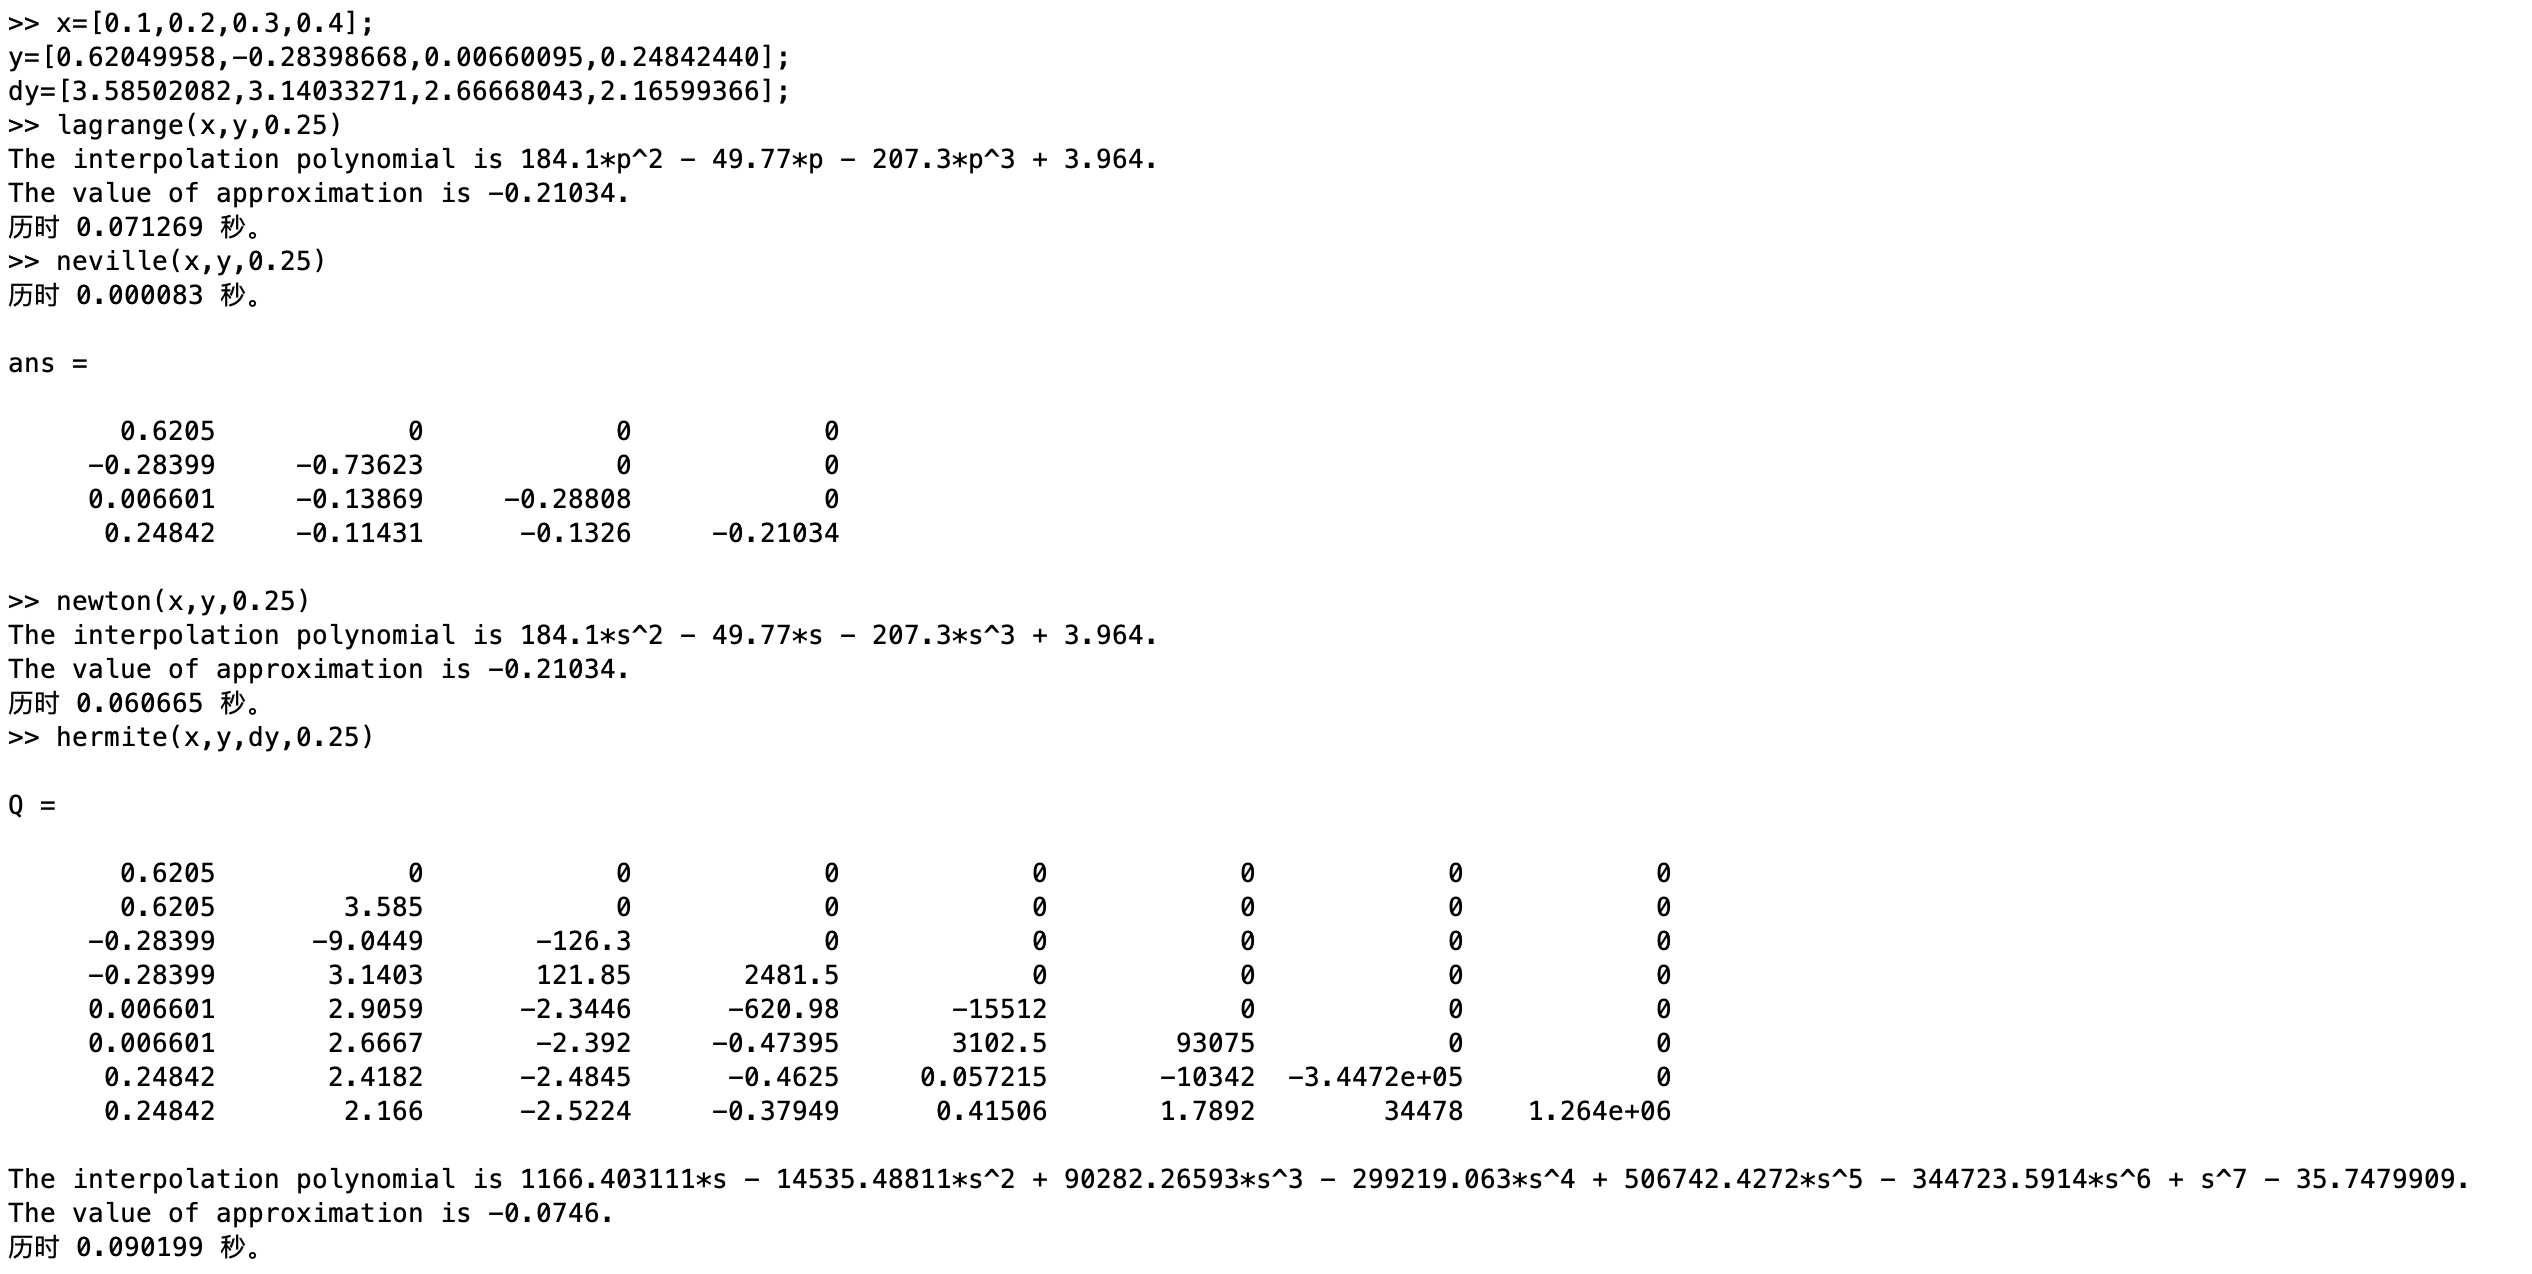
\includegraphics[scale=0.4]{Programme1}
    \end{figure}

    其中注意到前三个三个方程计算\textbf{所得结果相同},其原因为所用的插值多项式都为比数据的维度低一维的多项式(唯一性由数学定理保证)。最终逼近值为
    $$f(0.25)=-0.21034
    $$

    以及\textbf{唯一}的多项式(结果保留四位有效数字)
    $$f(x)=-207.3\cdot x^3+184.1\cdot x^2-49.77\cdot x+3.964.
    $$

    考察四个程序的CPU时间发现:Neville的计算时间最短,hermite由于加入导数的计算时间变长。其余两个处于中等水平且Newton由于迭代风格出众略居其上。

\subsection{2.2 程序说明}
    在Lagrange差值多项式与Nevile中都是循规蹈矩按照书上的程序图写下代码。但在第三个代码中,我们改进了书中的公式。计算所有形如:
    $$ f[x_{0},\ldots]
    $$
    的newton差分,发现也可以得到每一个ewton任意阶差分。例如具体在在代码中,有如下的迭代
    $$\text{coeff}(j)=\frac{y(j)-y(i)}{x(j)-x(i)};
    $$
    其中任意次迭代的coeff(变量)代表newton差分表这一列的每一个系数。
    因此有更高效的迭代公式路径,最终代码如下。
    \begin{lstlisting}
    % Newton's interpolatory divided difference fomula
    % t is coordinate number to be evaluated
    function output=newton(x,y,t)
    % Calculate runtime of the program
    tic;
    % initialize
    newpoly=y(1);
    syms s;
    % compute the dimension of x
    n=length(x);
    coeff=zeros(1,n);
    temp1=zeros(1,n);
    dxs=1;
    for i=1:n-1
        for j=i+1:n
            coeff(j)=(y(j)-y(i))/(x(j)-x(i));
        end
        temp1(i)=coeff(i+1);    % tempoary variable
        dxs=dxs*(s-x(i));
        newpoly=newpoly+temp1(i)*dxs;
        y=coeff;
    end
    % simplify the polynomial
    newpoly=simplify(newpoly);
    newpoly=vpa(newpoly,4);
    % output the evaluted number
    m=length(t);
    % temporary value
    temp=zeros(1,m);
    for i=1:m
        temp(i)=subs(newpoly,'s',t(i));
    end
    disp(['The interpolation polynomial is ',char(newpoly),'.']);
    disp(['The value of approximation is ',num2str(temp),'.']);
    toc;
    \end{lstlisting}
    结果显示最终仍得到正确的逼近值$f(0.25)=-0.21034
    $与逼近多项式
    $$f(x)=-207.3\cdot x^3+184.1\cdot x^2-49.77\cdot x+3.964.
    $$
    这说明上述改进是正确的。

\newpage

\section{3. 用Hermite插值计算3.3节1d题}

\subsection{3.1 程序运行}

    本节使用3.3节1d题的数据。注意:该数据在$x=0.1$与$x=0.2$处的函数值与3.1 节 3c 题的函数值是互为相反数的。因此不可以将该数据运行的Hermite插值算法与上题数据运行的剩余插值算法进行比较!(将该数据在$x=0.1$与$x=0.2$处的函数值取反就可以比较,比较结果见第二节。)
    用Hermite插值多项式去逼近任意$f(x)$处的值,运行程序的结果如下。
    \begin{figure}[h]
    \centering
    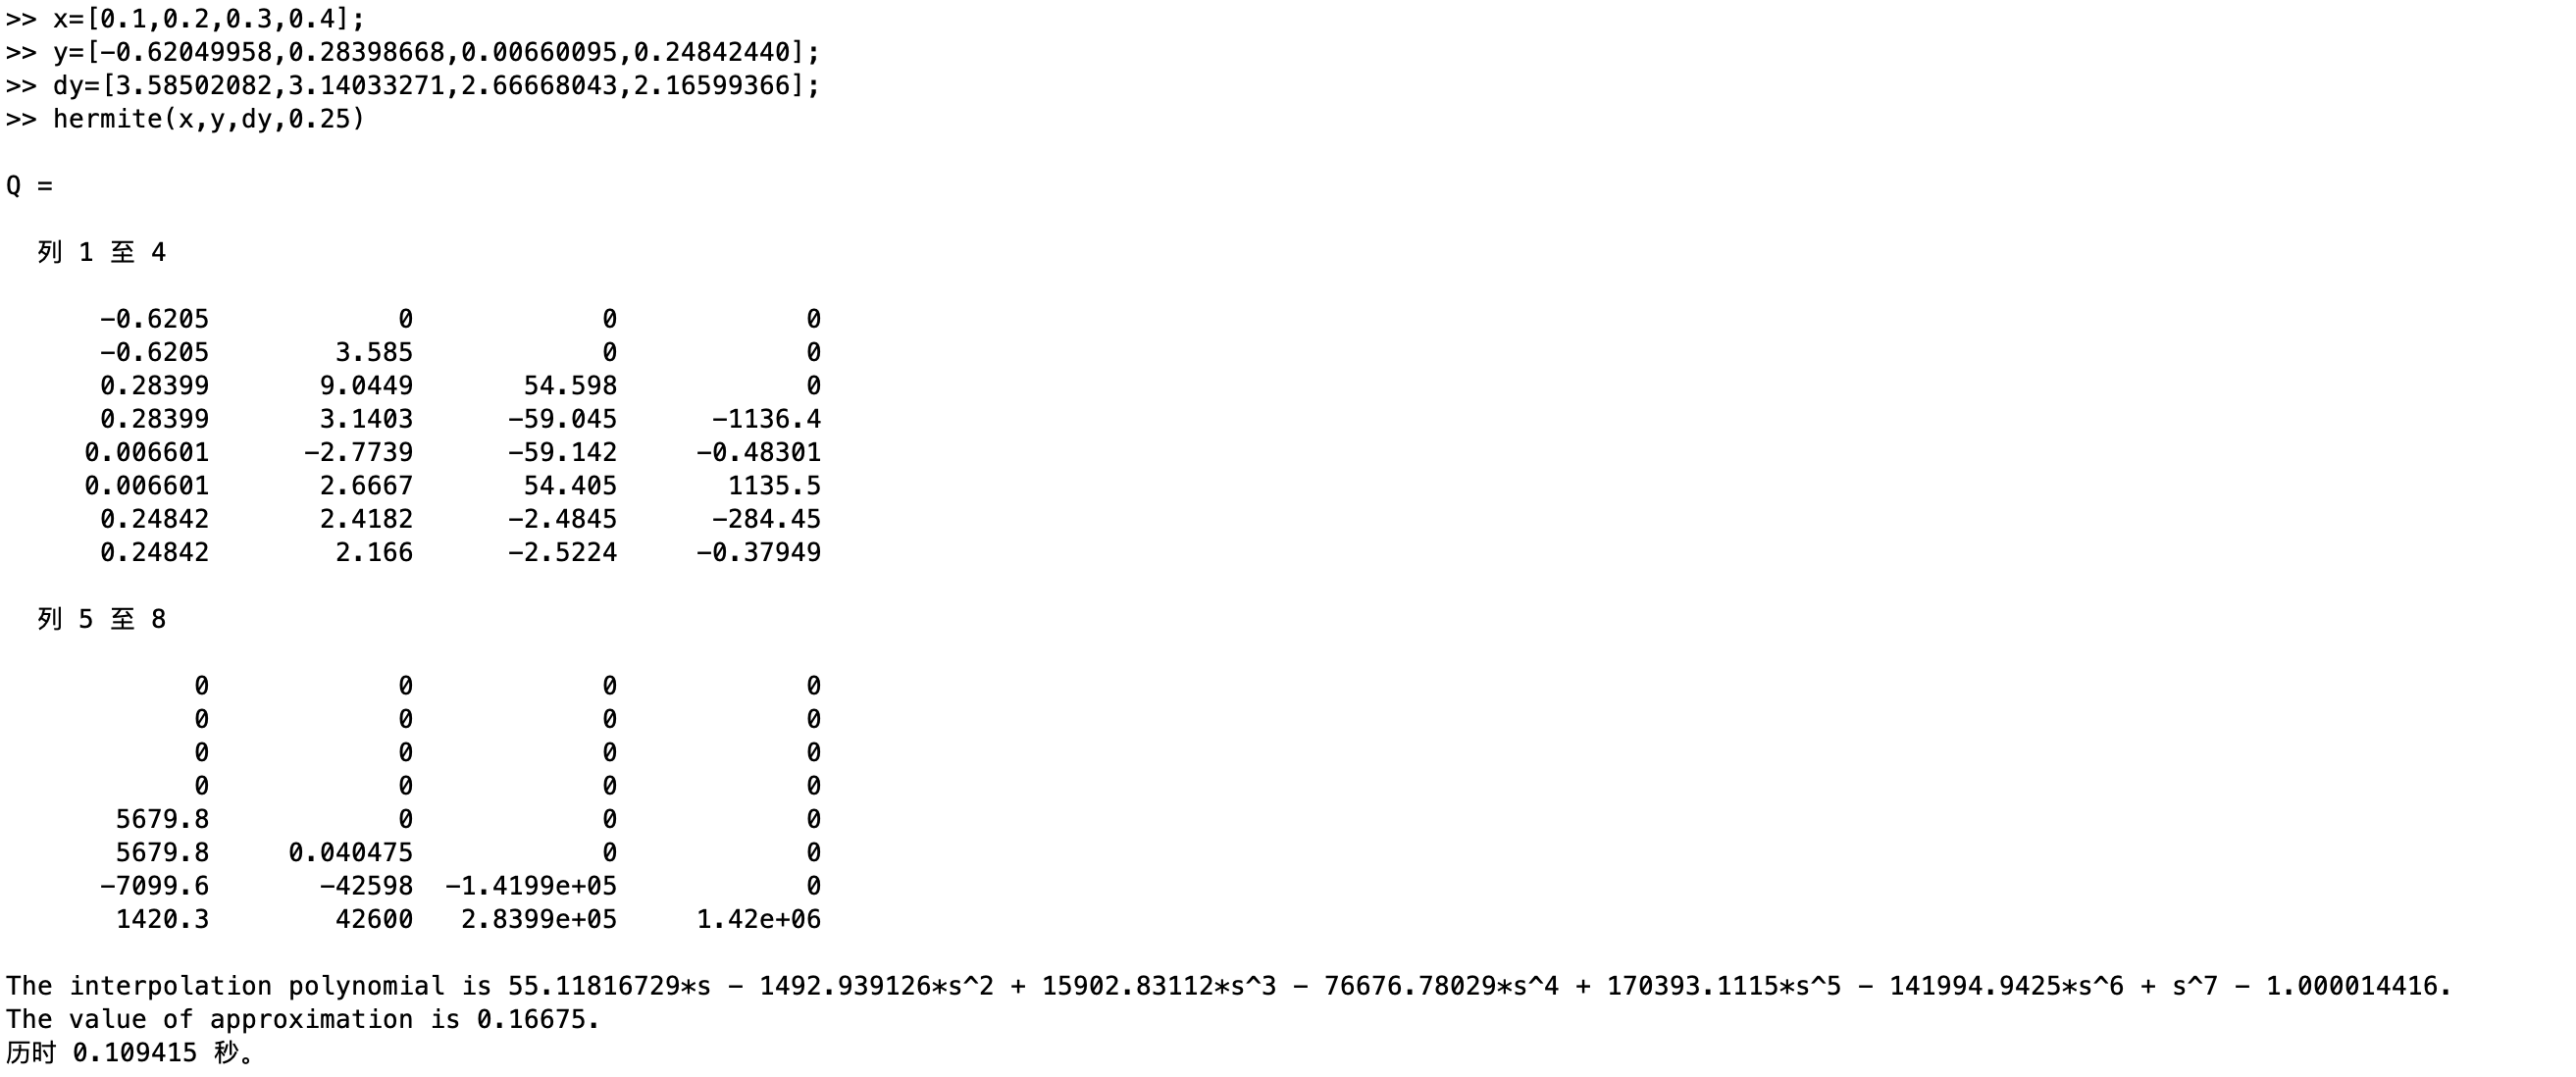
\includegraphics[scale=0.4]{Programme2}
    \end{figure}

    程序输出的是所有的Hermite多项式系数。最终得到逼近值为$f(0.25)=0.16675$。以及插值多项式,写成标准形式为:(保留10位有效数字)
    \begin{align*}
    f(s)=&55.11816729\cdot s - 1492.939126\cdot s^2 + 15902.83112\cdot s^3 - 76676.78029\cdot s^4 \\
    &+ 170393.1115\cdot s^5 - 141994.9425\cdot s^6 + s^7 - 1.000014416.
    \end{align*}

\subsection{3.2 程序分析}
    书中流程图的$x$下标由0开始,而\textbf{matlab的检索一般由1开始}。因此针对这个问题需要改进迭代公式,经过计算获得如下的迭代公式:
    $$Q(i,j)=\frac{Q(i,j-1)-Q(i-1,j-1)}{z(i)-z(i-j+1)}
    $$
    结果显示上述改进是正确的。

\subsection{3.3 试运行}
    虽说本段居于最后一节,但在逻辑上是首先的。由于该算法的迭代公式较为复杂,笔者运用所写算法去运行书中数据进行检验:考察\textbf{书中Table3.12}的数据,运行如下:
    \begin{figure}[h]
    \centering
    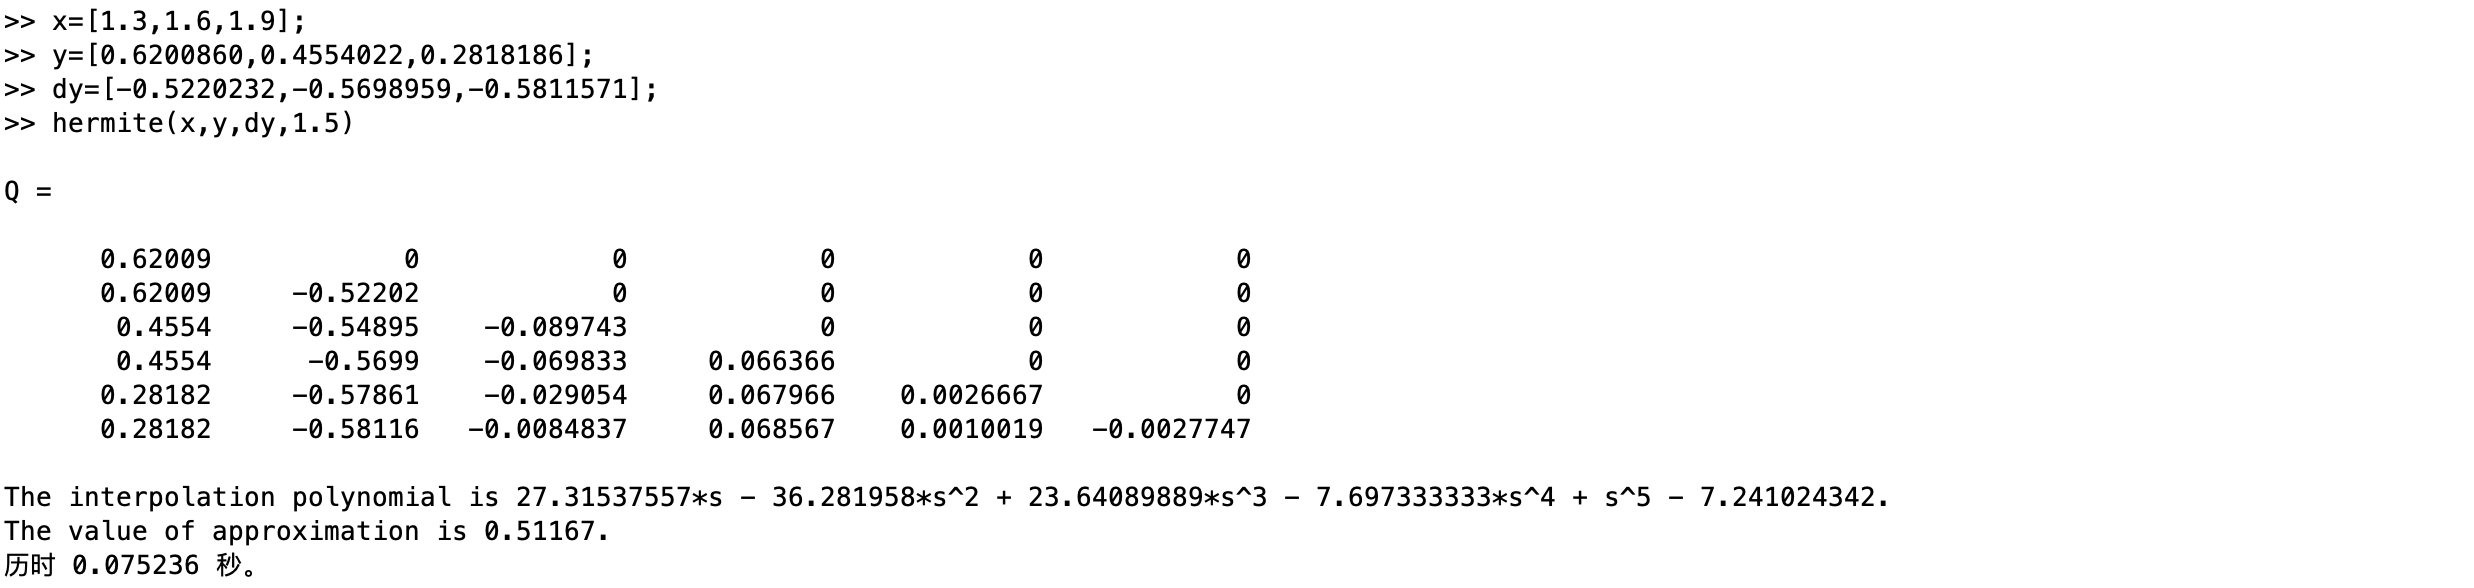
\includegraphics[scale=0.4]{Programme3}
    \end{figure}

\newpage

    与3.14进行比较发现\textbf{表格数据与最终拟合的数据完全一致},且逼近值
    $$f(0.25)=0.512=H_{5}(1.5)$$
    最终验证了所写算法的正确性!
   
\section{4. 代码附录}
    \subsection{4.1 Lagrange插值}
    \begin{lstlisting}
    % lagrange polynomial for interpolation
    % t is coordinate number (vector) to be evaluated
    function output=lagrange(x,y,t)
    % Calculate runtime of the program
    tic;
    % calculate the dimension of x
    n=length(x);
    syms p;
    % calulate the lagrange polynomial
    lapoly=0;
    for i=1:n
        labase=y(i);
        for j=1:i-1
            labase=labase*(p-x(j))/(x(i)-x(j));
        end
        for j=i+1:n
            labase=labase*(p-x(j))/(x(i)-x(j));
        end
        lapoly=lapoly+labase;
    end
    lapoly=simplify(lapoly);
    lapoly=vpa(lapoly,4);
    % output the evaluted number
    m=length(t);
    % temporary value
    temp=zeros(1,m);
    for i=1:m
        temp(i)=subs(lapoly,'p',t(i));
    end
    disp(['The interpolation polynomial is ',char(lapoly),'.']);
    disp(['The value of approximation is ',num2str(temp),'.']);
    toc;
    \end{lstlisting}

\subsection{4.2 Neville迭代插值}
    \begin{lstlisting}
    % neville's iterated interpolation 
    % t is coordinate number to be evaluated
    function output=neville(x,y,t)
    n=length(x);
    % Calculate runtime of the program
    tic;
    % initialize the table
    Q=zeros(n,n);
    for i=1:n
        Q(i,1)=y(i);
    end
    for i=2:n
        for k=2:i
            Q(i,k)=((t-x(i-k+1))*Q(i,k-1)-(t-x(i))*Q(i-1,k-1))/(x(i)-x(i-k+1));
        end
    end
    toc
    output=Q;
    \end{lstlisting}

    \subsection{4.3 Newton插值}
    \begin{lstlisting}
    % Newton's interpolatory divided difference fomula
    % t is coordinate number to be evaluated
    function output=newton(x,y,t)
    % Calculate runtime of the program
    tic;
    % initialize
    newpoly=y(1);
    syms s;
    % compute the dimension of x
    n=length(x);
    coeff=zeros(1,n);
    temp1=zeros(1,n);
    dxs=1;
    for i=1:n-1
        for j=i+1:n
            coeff(j)=(y(j)-y(i))/(x(j)-x(i));
        end
        temp1(i)=coeff(i+1);    % tempoary variable
        dxs=dxs*(s-x(i));
        newpoly=newpoly+temp1(i)*dxs;
        y=coeff;
    end
    % simplify the polynomial
    newpoly=simplify(newpoly);
    newpoly=vpa(newpoly,4);
    % output the evaluted number
    m=length(t);
    % temporary value
    temp=zeros(1,m);
    for i=1:m
        temp(i)=subs(newpoly,'s',t(i));
    end
    disp(['The interpolation polynomial is ',char(newpoly),'.']);
    disp(['The value of approximation is ',num2str(temp),'.']);
    toc;
    \end{lstlisting}

    \subsection{4.4 Hermite插值}
    \begin{lstlisting}
    % Hermite interpolation
    % t is coordinate number to be evaluated
    function output=hermite (x,y,dy,t)
    % Calculate runtime of the program
    tic;
    % compute the dimension of x
    n=length(x);
    syms s;
    z=zeros(2*n,1);
    Q=zeros(2*n,2*n);
    for i=1:n
        z(2*i-1)=x(i);
        z(2*i)=x(i);
        Q(2*i-1,1)=y(i);
        Q(2*i,1)=y(i);
        Q(2*i,2)=dy(i);
        if(i~=1)
            Q(2*i-1,2)=(Q(2*i-1,1)-Q(2*i-2,1))/(z(2*i-1)-z(2*i-2));
        end
    end
    for i=3:(2*n)
        for j=3:i
            Q(i,j)=(Q(i,j-1)-Q(i-1,j-1))/(z(i)-z(i-j+1));
        end
    end

    % compute the hermite poynomial
    temp=1;
    hermitepoly=Q(1,1);
    for i=1:n-1
        temp=temp*(s-x(i));
        hermitepoly=hermitepoly+Q(2*i,2*i)*temp;
        temp=temp*(s-x(i));
        hermitepoly=hermitepoly+Q(2*i+1,2*i+1)*temp;
    end
    hermitepoly=hermitepoly+temp*(s-x(n));
    hermitepoly=simplify(hermitepoly);
    hermitepoly=vpa(hermitepoly,10);
    % output the evaluted number
    m=length(t);
    % temporary value
    temp=zeros(1,m);
    for i=1:m
        temp(i)=subs(hermitepoly,'s',t(i));
    end
    Q
    disp(['The interpolation polynomial is ',char(hermitepoly),'.']);
    disp(['The value of approximation is ',num2str(temp),'.']);
    toc;
    \end{lstlisting}


\end{document}
